% Provenance (never printed): cycle 4 SVT/physique, "La planete Terre,
% l'environnement": the atmosphere, its structure and its layers, pressure
% and altitude, the ozone layer; see sources/book1/PROVENANCE.md. Book 1,
% grade 8, chapter 1.
% Vocabulary guard: owns the layers of the atmosphere (troposphere,
% tropopause, stratosphere, mesosphere, thermosphere), the environmental
% lapse rate and the ozone layer. Air pressure and the barometer are the
% physics books' (recalled), the composition of air and ozone the molecule
% the chemistry books'; "convection cell" is g8.2's and is not used here;
% adiabatic cooling is Book 2's.
\chapter{الغلاف الجوي}\label{ch:g8:the-atmosphere}

في \omterm{def:g4:clouds-rain-snow:weather-station}{محطة أرصاد جوية}، قبيل الساعة المتفق عليها، تخرج خبيرة أرصاد إلى العشب
وهي تمسك بالونًا مملوءًا بالهيدروجين أو الهيليوم، قطره نحو \qty{1.5}{m}.
وتحته، على خيط طويل، تتدلى مظلة صغيرة برتقالية وصندوق أجهزة يزن من 60 إلى
80 غرامًا: إنه \emph{المسبار اللاسلكي}. ثم تفلته. فيصعد البالون نحو
\qty{300}{m} كل دقيقة، ويرسل المسبار اللاسلكي كل ثانية بالراديو الضغط ودرجة
الحرارة والرطوبة وموقعه. وكلما ارتفع البالون انتفخ، حتى يبلغ قطره من 6 إلى
\qty{8}{m} فينفجر، وكثيرًا ما يكون ذلك على \omterm{def:g4:world-physical-map:altitude}{ارتفاع} يزيد على \qty{30}{km}،
بعد ساعتين من الإطلاق. وفي الساعات نفسها من كل يوم، يتكرر المشهد نفسه في
أكثر من 800 محطة حول العالم.
% ledger: nws:radiosonde

\begin{omfigure}
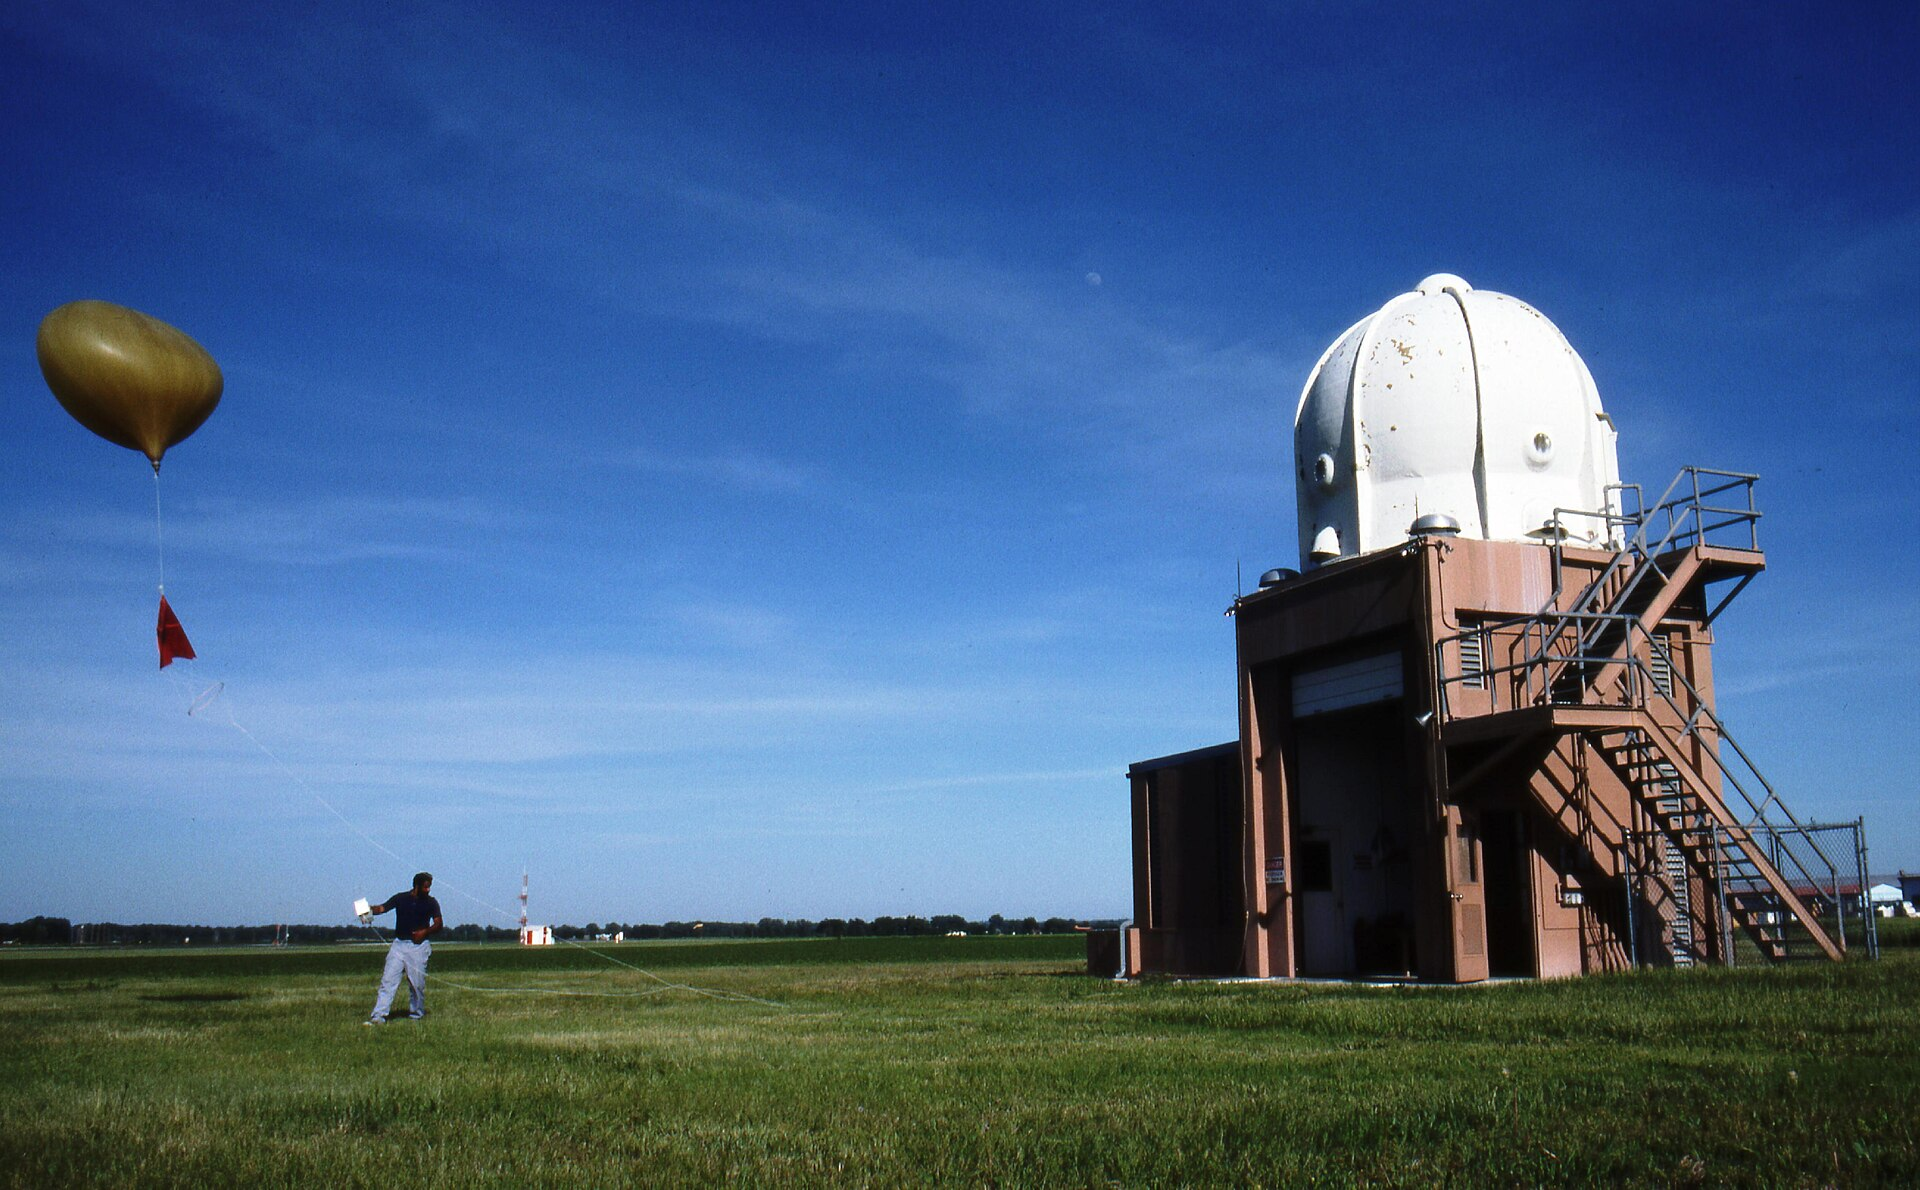
\includegraphics[width=0.78\linewidth]{images/book1/g8-radiosonde-launch.jpg}

{\small إطلاق بالون أرصاد في توبيكا، كانساس (الولايات المتحدة): المظلة
(بالأحمر) والمسبار اللاسلكي يتدليان تحت البالون. الصورة: ستيفن
كورفيدي، الإدارة الوطنية للمحيطات والغلاف الجوي، هيئة الأرصاد الجوية
الوطنية الأمريكية (ملك عام، عبر ويكيميديا كومنز).}
% ledger: commons:radiosonde-launch
\label{fig:g8:the-atmosphere:launch}
\end{omfigure}

لماذا ينتفخ البالون كلما ارتفع؟ وماذا يقيس المسبار اللاسلكي في طريقه إلى
الأعلى، ولماذا لا تواصل درجة الحرارة الانخفاض ببساطة؟ وأين ينتهي
الهواء؟

\begin{recall}
\emph{الغلاف الجوي} هو طبقة الهواء المحيطة بالأرض. والهواء يضغط على كل
ما يلامسه: هذا هو \emph{الضغط الجوي}، ويُقاس بالبارومتر (كتب الفيزياء).
وتعطيه هيئات الأرصاد بالهكتوباسكال \babelsublr{(hPa)}؛ وهو عند \omterm{def:g4:world-physical-map:altitude}{مستوى سطح
البحر} نحو \qty{1013}{hPa}. ويتكون الهواء الجاف من نحو 78~\% من النيتروجين
و21~\% من الأكسجين، مع قليل من الأرغون وثاني أكسيد الكربون وغازات أخرى
(كتب الكيمياء). \omterm{def:g4:clouds-rain-snow:cloud}{والسحب} مكوَّنة من قطيرات ماء دقيقة أو من بلورات جليد
(\cref{ch:g4:clouds-rain-snow}).
\end{recall}
% ledger: air:N2, air:O2, ussa76:sea-level

\section{غلاف رقيق}

إذا نُظر إلى الغلاف الجوي من محطة الفضاء الدولية، بدا خطًا رقيقًا متوهجًا
على طول حافة الأرض. ومعظم الهواء، وكل \omterm{def:g4:clouds-rain-snow:cloud}{السحب} تقريبًا، في كيلومتراته
القليلة السفلى.
% ledger: commons:iss-sunset

\begin{omfigure}
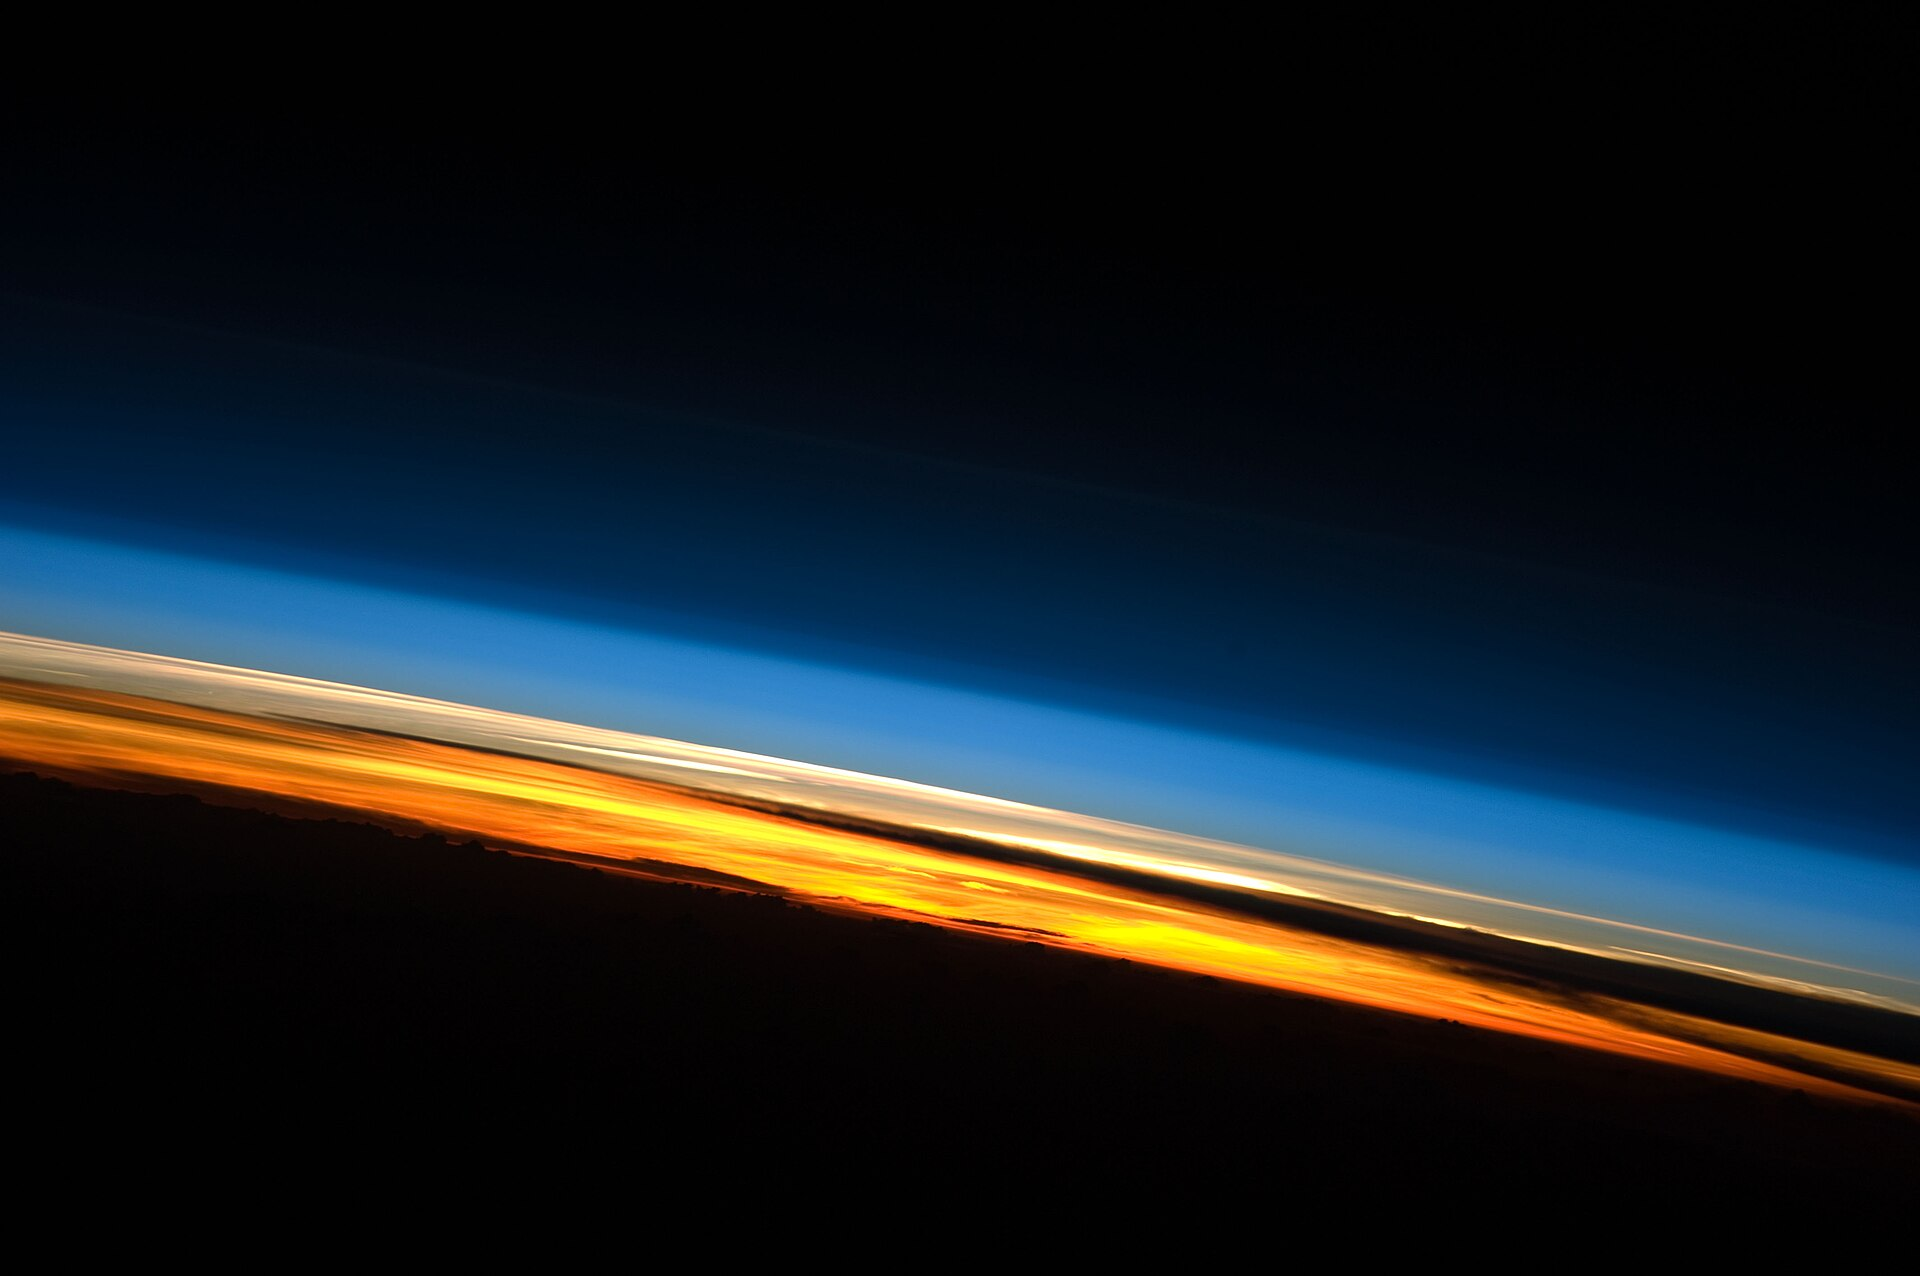
\includegraphics[width=0.78\linewidth]{images/book1/g8-iss-limb.jpg}

{\small حافة الأرض عند الغروب، مصوَّرة من محطة الفضاء الدولية فوق \omterm{def:g2:water-on-earth:ocean}{المحيط}
الهندي في 14~يونيو 2010. والشريط البرتقالي والأصفر هو الطبقة السفلى من
الغلاف الجوي، بسحبها الداكنة؛ وفوقه طبقات أشحب ثم زرقاء، تتلاشى في سواد
الفضاء. صورة وكالة ناسا، البعثة~23 إلى محطة الفضاء الدولية (ملك عام، عبر
ويكيميديا كومنز).}
% ledger: commons:iss-sunset
\label{fig:g8:the-atmosphere:limb}
\end{omfigure}

ليس للغلاف الجوي سطح علوي حاد: فالهواء يزداد خفة كلما ارتفعنا. وقد
اتُّفق على أن الفضاء يبدأ على \omterm{def:g4:world-physical-map:altitude}{ارتفاع} نحو \qty{100}{km}. وهذا قليل جدًا
مقارنة بنصف قطر الأرض، \qty{6371}{km}: $100 \div
6371 \approx 0.016$، أي أقل من 2~\% من نصف القطر. وعلى \omterm{def:g3:continents-and-oceans:globe}{مجسم كرة أرضية}
قطره \qty{30}{cm}، يكون الغلاف الجوي كله غشاء سماكته نحو
\qty{2}{mm}.
% ledger: ucar:layers, earth:Rmean

\begin{omfigure}
\begin{tikzpicture}[font=\footnotesize]
  % 1 cm = 100 km: the Earth's surface is a circle of radius 63.71 cm
  \def\R{63.71}
  \useasboundingbox (-6.9,-1.6) rectangle (6.9,1.0);
  \fill[blue!8] (0,-\R) ++(85:\R+1) arc (85:95:\R+1) -- ($(0,-\R)+(95:\R)$) arc (95:85:\R) -- cycle;
  \fill[omLithAlluv!70] (0,-\R) ++(85:\R) arc (85:95:\R) -- ++(0,-0.6) -- ($(0,-\R)+(85:\R)+(0,-0.6)$) -- cycle;
  \draw[black, line width=0.6pt] (0,-\R) ++(85:\R) arc (85:95:\R);
  \foreach \h/\c in {0.1102/omThm, 0.4938/omMeth, 0.86/omDef} \draw[\c, line width=0.5pt] (0,-\R) ++(85:\R+\h) arc (85:95:\R+\h);
  \draw[black!60, dashed] (0,-\R) ++(85:\R+1) arc (85:95:\R+1);
  \node[anchor=west, omThm] at (5.65,-0.14) {\qty{11}{km}};
  \node[anchor=west, omMeth] at (5.65,0.25) {\qty{49}{km}};
  \node[anchor=west, omDef] at (5.65,0.62) {\qty{86}{km}};
  \node[anchor=east, black!70] at (-5.65,0.75) {\qty{100}{km}};
  \node[anchor=north] at (0,-0.15) {سطح الأرض};
  \draw[|-|] (-5,-1.05) -- node[below] {\qty{1000}{km}} (5,-1.05);
\end{tikzpicture}

{\small شريحة من الأرض وغلافها الجوي مرسومة بمقياس رسم
(\qty{1}{cm} لكل \qty{100}{km})، حتى \qty{100}{km}، أي حافة الفضاء
(الخط المتقطع). والخطوط الملونة حدود الطبقات التي سنتعرف عليها لاحقًا في
هذا الفصل؛ والطبقة السفلى، التي يحدث فيها كل \omterm{def:g1:watching-the-weather:weather}{الطقس}، لا تكاد سماكتها
تبلغ مليمترًا.}
% ledger: earth:Rmean, ucar:layers (limits: figdata/grade-8/standard_atmosphere.py main table)
\label{fig:g8:the-atmosphere:to-scale}
\end{omfigure}

\section{الضغط ينخفض مع الارتفاع}

يحمل الهواء في أسفل الغلاف الجوي ثقل كل الهواء الذي فوقه. وكلما صعدنا
أعلى، قل الهواء الباقي فوق رؤوسنا، وانخفض الضغط. وفي النموذج المعياري
للغلاف الجوي الذي يستعمله خبراء الأرصاد والمهندسون، يبلغ الضغط
\qty{1013}{hPa} عند \omterm{def:g4:world-physical-map:altitude}{مستوى سطح البحر}، ونصف ذلك على \omterm{def:g4:world-physical-map:altitude}{ارتفاع} نحو
\qty{5.5}{km}، وربعه على \omterm{def:g4:world-physical-map:altitude}{ارتفاع} نحو \qty{10.3}{km}.
% ledger: ussa76:sea-level, ussa76:layers (figdata/grade-8/standard_atmosphere.py main table: half_km 5.48, quarter_km 10.29)

بما أن الضغط يقيس ثقل الهواء الذي فوق، فإن مستوى نصف الضغط هو أيضًا
\omterm{def:g4:world-physical-map:altitude}{الارتفاع} الذي يقع تحته نصف الهواء كله: فنصف الغلاف الجوي محشور في
\qty{5.5}{km} السفلى منه. وتحت \qty{11}{km} يقع نحو 78~\% من الهواء،
وتحت \qty{30}{km} نحو 99~\%.
% ledger: (computed: figdata/grade-8/standard_atmosphere.py, share_below_11km 77.7, share_below_30km 98.82)

\begin{omfigure}
\begin{minipage}[t]{0.49\linewidth}\centering
\begin{tikzpicture}
\begin{axis}[width=6.6cm, height=7.6cm, xmin=0, xmax=1100, ymin=0, ymax=30,
  xlabel={\foreignlanguage{arabic}{الضغط \babelsublr{(hPa)}}}, ylabel={\foreignlanguage{arabic}{الارتفاع \babelsublr{(km)}}},
  tick label style={font=\scriptsize}, label style={font=\small},
  xtick={0,250,500,750,1000}, ytick={0,5,10,15,20,25,30}]
  \addplot[dashed, black!60] table {figdata/out/grade-8-standard_atmosphere-guides.dat};
  \addplot[omDef, line width=1.1pt] table[x=p_hPa, y=z_km] {figdata/out/grade-8-standard_atmosphere-pressure.dat};
  \addplot[only marks, mark=*, mark size=1.8pt, omThm] table[x=p_hPa, y=z_km] {figdata/out/grade-8-standard_atmosphere-levels.dat};
  \node[anchor=south west, font=\scriptsize, text=black] at (axis cs:506.6,5.48) {النصف};
  \node[anchor=south west, font=\scriptsize, text=black] at (axis cs:253.3,10.29) {الربع};
\end{axis}
\end{tikzpicture}

{\small الضغط بحسب \omterm{def:g4:world-physical-map:altitude}{الارتفاع}. يبلغ الضغط نصف قيمته عند \omterm{def:g4:world-physical-map:altitude}{مستوى سطح البحر} على
\omterm{def:g4:world-physical-map:altitude}{ارتفاع} نحو \qty{5.5}{km}، وربعها على \omterm{def:g4:world-physical-map:altitude}{ارتفاع} نحو \qty{10.3}{km}.}
\end{minipage}\hfill
\begin{minipage}[t]{0.49\linewidth}\centering
\begin{tikzpicture}[font=\footnotesize]
  % at launch: 1.5 m; at burst: about 7 m (drawn 1 cm for 1.5 m)
  \draw[black!60] (0,0.9) -- (0,2.6);
  \shade[ball color=yellow!60!brown] (0,3.1) circle (0.5);
  \fill[red!75] (-0.25,1.75) .. controls (-0.2,2.05) and (0.2,2.05) .. (0.25,1.75) -- cycle;
  \fill[white, draw=black] (-0.15,0.55) rectangle (0.15,0.9);
  \node[anchor=north] at (0,0.45) {عند الإطلاق};
  \node[anchor=north] at (0,0.05) {\foreignlanguage{arabic}{قطره \babelsublr{\qty{1.5}{m}}}};
  \begin{scope}[xshift=3.1cm]
    \draw[black!60] (0,0.9) -- (0,2.6);
    \shade[ball color=yellow!40!white] (0,4.9) circle (2.3);
    \fill[red!75] (-0.25,1.75) .. controls (-0.2,2.05) and (0.2,2.05) .. (0.25,1.75) -- cycle;
    \fill[white, draw=black] (-0.15,0.55) rectangle (0.15,0.9);
    \node[anchor=north] at (0,0.45) {قبيل انفجاره};
    \node[anchor=north] at (0,0.05) {\foreignlanguage{arabic}{قطره من \babelsublr{6} إلى \babelsublr{\qty{8}{m}}}};
  \end{scope}
  \node[anchor=west, font=\scriptsize] at (0.3,1.9) {المظلة};
  \node[anchor=west, font=\scriptsize] at (0.3,0.72) {المسبار اللاسلكي};
\end{tikzpicture}

{\small ينتفخ البالون كلما صعد، لأن الهواء \omterm{def:g2:water-on-earth:ocean}{المحيط} به يضغط عليه أقل فأقل
(البالونان والمظلتان بمقياس رسم واحد بعضها لبعض، والخيط
مقصَّر).}
% ledger: nws:radiosonde
\end{minipage}
% ledger: ussa76:sea-level, ussa76:layers (figdata/grade-8/standard_atmosphere.py parts pressure, levels, guides)
\label{fig:g8:the-atmosphere:pressure}
\end{omfigure}

وفي الأعلى، يواصل الضغط الانخفاض، فينقص إلى النصف تقريبًا مرة أخرى كل بضعة
كيلومترات، فلا يلبث أن يصير ضئيلًا جدًا. وقوى العشرة أفضل طريقة لكتابته. فعلى
\omterm{def:g4:world-physical-map:altitude}{ارتفاع} \qty{30}{km}، يبلغ الضغط نحو \qty{12}{hPa}، أي قرابة
$10^{-2}$ من قيمته عند \omterm{def:g4:world-physical-map:altitude}{مستوى سطح البحر} (جزء من مئة)؛ وعلى \omterm{def:g4:world-physical-map:altitude}{ارتفاع} \qty{50}{km}، نحو
\qty{0.8}{hPa}، أي قرابة $10^{-3}$؛ وعلى \omterm{def:g4:world-physical-map:altitude}{ارتفاع} \qty{80}{km}، نحو
\qty{0.01}{hPa}، أي قرابة $10^{-5}$ من الضغط عند \omterm{def:g4:world-physical-map:altitude}{مستوى سطح البحر}.
% ledger: ussa76:layers (figdata/grade-8/standard_atmosphere.py main table: p_30km 11.97, p_50km 0.798, p_80km 0.0105 hPa)

\begin{omfigure}
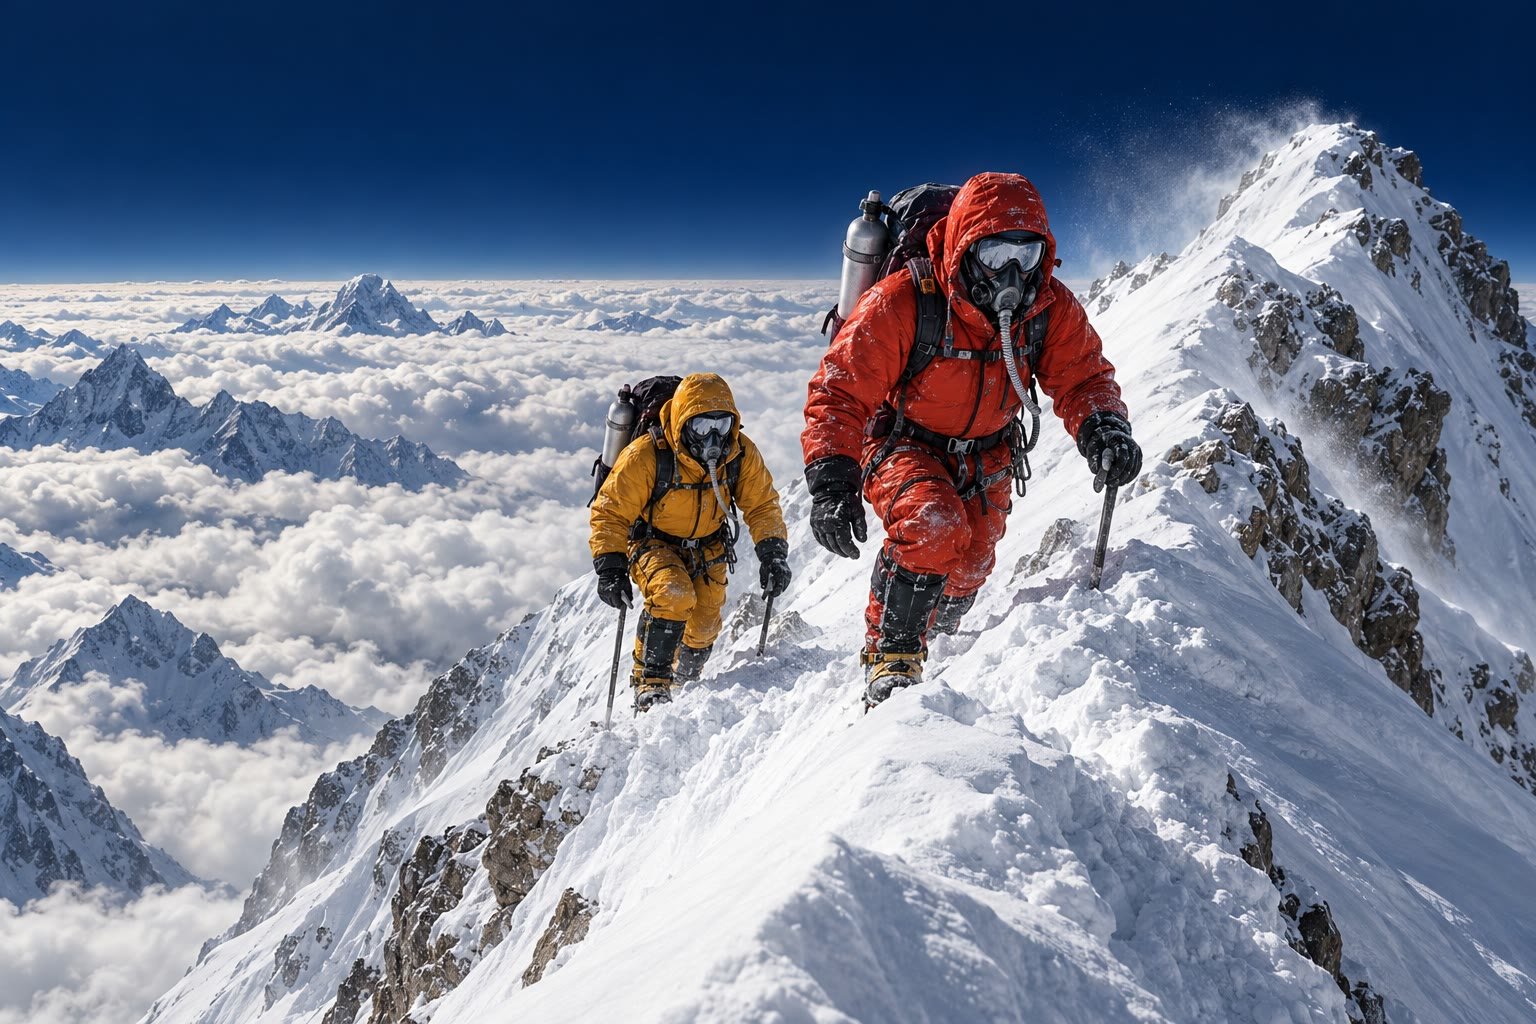
\includegraphics[width=0.5\linewidth]{images/book1/ai/g8-climbers.jpg}

{\small متسلقون على \omterm{def:g1:landscapes-around-us:landform}{جبل} شاهق جدًا يحملون قوارير أكسجين. فعلى \omterm{def:g4:world-physical-map:altitude}{ارتفاع}
\qty{9}{km}، يقل الضغط عن ثلث قيمته عند \omterm{def:g4:world-physical-map:altitude}{مستوى سطح البحر}: فالهواء لا يزال
يحوي 21~\% من الأكسجين، لكن كل نفَس يُدخل منه أقل بكثير (رسم توضيحي
مولَّد بالذكاء الاصطناعي لمشهد عام).}
% ledger: air:O2 (figdata/grade-8/standard_atmosphere.py: pressure at 9 km 308 hPa, 30 % of sea level)
\label{fig:g8:the-atmosphere:climbers}
\end{omfigure}

\section{درجة الحرارة والطبقات}

كل من تسلق جبلًا يعرف أن الهواء يزداد برودة مع \omterm{def:g4:world-physical-map:altitude}{الارتفاع}. لكن المسابير
اللاسلكية تبين أن هذا لا يصح إلا في الجزء الأسفل من الغلاف الجوي. ففي
الأعلى، تتوقف درجة الحرارة عن الانخفاض، ثم ترتفع، ثم تنخفض من جديد، ثم
ترتفع مرة أخرى. وهذه التغيرات تقسم الغلاف الجوي إلى طبقات.
% ledger: ucar:layers, ussa76:layers

\begin{omfigure}
\begin{tikzpicture}
\begin{axis}[width=10cm, height=9cm, xmin=-100, xmax=30, ymin=0, ymax=100,
  xlabel={\foreignlanguage{arabic}{درجة الحرارة \babelsublr{($^\circ$C)}}}, ylabel={\foreignlanguage{arabic}{الارتفاع \babelsublr{(km)}}},
  tick label style={font=\scriptsize}, label style={font=\small},
  xtick={-100,-80,-60,-40,-20,0,20}, ytick={0,10,20,30,40,50,60,70,80,90,100}, axis on top]
  \addplot[fill=omSea!55, draw=none] table {figdata/out/grade-8-standard_atmosphere-band-troposphere.dat};
  \addplot[fill=omMeth!12, draw=none] table {figdata/out/grade-8-standard_atmosphere-band-stratosphere.dat};
  \addplot[fill=omSea!35, draw=none] table {figdata/out/grade-8-standard_atmosphere-band-mesosphere.dat};
  \addplot[fill=omThm!10, draw=none] table {figdata/out/grade-8-standard_atmosphere-band-thermosphere.dat};
  \addplot[omThm, line width=1.2pt] table[x=T_C, y=z_km] {figdata/out/grade-8-standard_atmosphere-temp.dat};
  \node[anchor=west, font=\small\bfseries, text=black!75] at (axis cs:-97,5.51) {التروبوسفير};
  \node[anchor=west, font=\small\bfseries, text=black!75] at (axis cs:-97,30.2) {الستراتوسفير};
  \node[anchor=west, font=\small\bfseries, text=black!75] at (axis cs:-97,67.69) {الميزوسفير};
  \node[anchor=west, font=\small\bfseries, text=black!75] at (axis cs:-60,93) {الثرموسفير};
  \draw[black!50, dashed] (axis cs:-100,11.02) -- (axis cs:30,11.02);
  \draw[black!50, dashed] (axis cs:-100,49.38) -- (axis cs:30,49.38);
  \draw[black!50, dashed] (axis cs:-100,86) -- (axis cs:30,86);
  \node[anchor=south east, font=\scriptsize] at (axis cs:17,11.02) {التروبوبوز};
  \node[anchor=south east, font=\scriptsize] at (axis cs:29,49.38) {الستراتوبوز};
  \node[anchor=south east, font=\scriptsize] at (axis cs:29,86) {الميزوبوز};
  \fill[omMeth!45] (axis cs:19,16) rectangle (axis cs:23,48);
  \node[anchor=east, font=\scriptsize, align=right] at (axis cs:18,30) {طبقة\\الأوزون};
\end{axis}
\end{tikzpicture}

{\small درجة حرارة الهواء بحسب \omterm{def:g4:world-physical-map:altitude}{الارتفاع}، من الأرض حتى \qty{100}{km}، في
الغلاف الجوي المعياري (متوسط للعروض الوسطى). والطبقات الأربع مظللة؛
والشريط الأخضر يحدد \omterm{def:g4:world-physical-map:altitude}{ارتفاع} \omterm{def:g8:the-atmosphere:ozone-layer}{طبقة الأوزون}.}
% ledger: ussa76:sea-level, ussa76:layers, ussa76:above-86, ucar:ozone (figdata/grade-8/standard_atmosphere.py parts temp, layers, band-*)
\label{fig:g8:the-atmosphere:temperature}
\end{omfigure}

\begin{definition}[طبقات الغلاف الجوي]\label{def:g8:the-atmosphere:layers}
من الأرض إلى الأعلى، ينقسم الغلاف الجوي إلى أربع طبقات بحسب طريقة تغير
درجة حرارته مع \omterm{def:g4:world-physical-map:altitude}{الارتفاع}:
\begin{itemize}
  \item \emph{التروبوسفير}\index{تروبوسفير}، حيث تنخفض درجة الحرارة مع
        \omterm{def:g4:world-physical-map:altitude}{الارتفاع} وحيث يحدث \omterm{def:g1:watching-the-weather:weather}{الطقس} كله تقريبًا؛ وحده العلوي هو
        \emph{التروبوبوز}\index{تروبوبوز}؛
  \item \emph{الستراتوسفير}\index{ستراتوسفير}، حيث ترتفع درجة الحرارة مع
        \omterm{def:g4:world-physical-map:altitude}{الارتفاع}، حتى نحو \qty{50}{km}؛
  \item \emph{الميزوسفير}\index{ميزوسفير}، حيث تنخفض درجة الحرارة من
        جديد، حتى نحو \qty{85}{km}؛
  \item \emph{الثرموسفير}\index{ثرموسفير}، حيث يزداد الهواء الشديد الخفة
        حرارة كلما ارتفعنا.
\end{itemize}
\end{definition}
% ledger: ucar:layers, ussa76:layers

يحوي \omterm{def:g8:the-atmosphere:layers}{التروبوسفير} نحو 99~\% من بخار الماء في الغلاف الجوي، ولذلك تتكون فيه
كل \omterm{def:g4:clouds-rain-snow:cloud}{السحب} والأمطار والثلوج تقريبًا. وهواؤه يُقلَّب طوال الوقت. وليس أعلى
\omterm{def:g8:the-atmosphere:layers}{التروبوسفير} على \omterm{def:g4:world-physical-map:altitude}{الارتفاع} نفسه في كل مكان: \omterm{def:g8:the-atmosphere:layers}{فالتروبوبوز} أعلى ما يكون فوق
\omterm{def:g3:continents-and-oceans:equator}{خط الاستواء}، حيث قد يبلغ \qty{20}{km}، وأدنى ما يكون فوق \omterm{def:g3:continents-and-oceans:poles}{القطبين}، حيث قد
ينزل إلى \qty{7}{km} في الشتاء. وهو أيضًا أعلى في الصيف منه في الشتاء. وفي
الغلاف الجوي المعياري، وهو متوسط للعروض الوسطى، يقع على \omterm{def:g4:world-physical-map:altitude}{ارتفاع} \qty{11}{km}.
% ledger: ucar:layers, ucar:tropopause, ussa76:layers

\begin{definition}[معدل التناقص الحراري البيئي]\label{def:g8:the-atmosphere:lapse-rate}
\emph{معدل التناقص الحراري البيئي}\index{معدل تناقص حراري بيئي} هو
المعدل الذي تنخفض به درجة حرارة الهواء مع \omterm{def:g4:world-physical-map:altitude}{الارتفاع} في \omterm{def:g8:the-atmosphere:layers}{التروبوسفير}، بالدرجات
المئوية لكل كيلومتر. وهو يتغير من يوم إلى يوم ومن مكان إلى آخر؛ ويستعمل
الغلاف الجوي المعياري متوسطًا قدره \qty{6.5}{\degreeCelsius} لكل
كيلومتر.
\end{definition}
% ledger: ussa76:layers

\begin{method}[قراءة مخطط درجة الحرارة]\label{met:g8:the-atmosphere:profile}
\begin{enumerate}
  \item جد \omterm{def:g4:world-physical-map:altitude}{الارتفاع} على المحور الرأسي وامضِ أفقيًا حتى المنحنى؛ ثم اقرأ
        درجة الحرارة تحته.
  \item حيث يميل المنحنى إلى اليسار وهو يصعد، يبرد الهواء مع \omterm{def:g4:world-physical-map:altitude}{الارتفاع}؛
        وحيث يميل إلى اليمين، يسخن الهواء مع \omterm{def:g4:world-physical-map:altitude}{الارتفاع}؛ وحيث يكون رأسيًا،
        لا تتغير درجة الحرارة.
  \item الحدود بين الطبقات هي حيث ينعطف المنحنى.
\end{enumerate}
\end{method}

\begin{example}[طائرة ركاب على ارتفاع التحليق]\label{ex:g8:the-atmosphere:airliner}
تحلّق طائرة ركاب على \omterm{def:g4:world-physical-map:altitude}{ارتفاع} \qty{11}{km}، قرب \omterm{def:g8:the-atmosphere:layers}{التروبوبوز}. وعلى المخطط،
تبلغ درجة الحرارة هناك نحو \qty{-56}{\degreeCelsius}. وبمعدل التناقص: من
\qty{15}{\degreeCelsius} عند \omterm{def:g4:world-physical-map:altitude}{مستوى سطح البحر}، يبرد الهواء
بمقدار $6.5 \times 11 = 71.5$ درجة، مما يعطي $15 - 71.5 =
\qty{-56.5}{\degreeCelsius}$. وعلى منحنى الضغط، يبلغ الضغط
نحو \qty{227}{hPa}، أي أقل من ربع الضغط على الأرض:
ولذلك يجب أن تُضغط المقصورة.
% ledger: ussa76:sea-level, ussa76:layers (figdata/grade-8/standard_atmosphere.py: T at 11 km -56.4 degC, p 227 hPa)
\end{example}

فوق \omterm{def:g8:the-atmosphere:layers}{التروبوبوز}، في \omterm{def:g8:the-atmosphere:layers}{الستراتوسفير}، تجد طائرات الركاب رحلة أهدأ: فالهواء
هناك يسخن مع \omterm{def:g4:world-physical-map:altitude}{الارتفاع}، فلا يُقلَّب من الأسفل. وفي \omterm{def:g8:the-atmosphere:layers}{الميزوسفير} تحترق معظم
الشهب، وفي أعلاه، قرب \qty{86}{km}، يوجد أبرد هواء في الغلاف الجوي كله،
نحو \qty{-86}{\degreeCelsius}. وفي \omterm{def:g8:the-atmosphere:layers}{الثرموسفير}، تسخّن الأشعة السينية
والأشعة فوق البنفسجية الآتية من الشمس الهواءَ الشديد الخفة إلى مئات
الدرجات، بل إلى آلافها أحيانًا؛ ومع ذلك فالهواء هناك قليل جدًا حتى إنه
لا يُحس حارًا. وكثير من الأقمار الصناعية تدور حول الأرض هناك.
% ledger: ucar:layers, ussa76:above-86

\section{طبقة الأوزون}

يسخن \omterm{def:g8:the-atmosphere:layers}{الستراتوسفير} مع \omterm{def:g4:world-physical-map:altitude}{الارتفاع} لأنه يمتص جزءًا من ضوء الشمس. والغاز الذي
يقوم بمعظم ذلك هو الأوزون، وهو شكل من أشكال الأكسجين (وكيمياؤه في كتب
الكيمياء).

\begin{definition}[طبقة الأوزون]\label{def:g8:the-atmosphere:ozone-layer}
\emph{طبقة الأوزون}\index{طبقة الأوزون} هي جزء \omterm{def:g8:the-atmosphere:layers}{الستراتوسفير} الواقع بين
نحو \qty{16}{km} و\qty{48}{km}، حيث يوجد نحو 90~\% من أوزون الغلاف الجوي.
وهي تمتص معظم الأشعة فوق البنفسجية الضارة الآتية من الشمس.
\end{definition}
% ledger: ucar:ozone

حتى في \omterm{def:g8:the-atmosphere:ozone-layer}{طبقة الأوزون}، الأوزون نادر: فليس منه إلا من 1 إلى 10 جزيئات في كل
مليون. ومع ذلك فهو، مع الأكسجين، يوقف ما بين 95~\% و99.9~\% من الأشعة فوق
البنفسجية التي تبلغ الأرض، ومنها أشد أنواعها ضررًا. والطاقة التي يمتصها
تتحول إلى حرارة، ولهذا ترتفع درجة الحرارة عبر \omterm{def:g8:the-atmosphere:layers}{الستراتوسفير}. ولولا \omterm{def:g8:the-atmosphere:ozone-layer}{طبقة
الأوزون}، لأضرت الأشعة فوق البنفسجية التي تبلغ الأرض بالكائنات الحية.
% ledger: ucar:ozone

\begin{inthefield}[تتبُّع بالونات الأرصاد]
تنشر هيئات الأرصاد قياسات مسابيرها اللاسلكية، وكثيرًا ما يكون ذلك في صورة
مخطط لدرجة الحرارة بحسب الارتفاع لكل إطلاق. ومع شخص بالغ، ابحث عن
مسابير المحطة الأقرب إليك، التي تُطلق في الساعة \babelsublr{00:00} أو
\babelsublr{12:00} بالتوقيت العالمي المنسق. وجد \omterm{def:g4:world-physical-map:altitude}{الارتفاع} الذي تتوقف عنده
درجة الحرارة عن الانخفاض: ذلك هو \omterm{def:g8:the-atmosphere:layers}{التروبوبوز} في ذلك اليوم. وقارن مسبارًا
شتويًا بمسبار صيفي.
\end{inthefield}
% ledger: nws:radiosonde, ucar:tropopause

\section{تمارين}

\begin{exercise}[$\star$]\label{exo:g8:the-atmosphere:1}
صِل كل طبقة بوصفها: \omterm{def:g8:the-atmosphere:layers}{التروبوسفير}؛ \omterm{def:g8:the-atmosphere:layers}{الستراتوسفير}؛ \omterm{def:g8:the-atmosphere:layers}{الميزوسفير}؛ \omterm{def:g8:the-atmosphere:layers}{الثرموسفير}.
(أ) ترتفع فيها درجة الحرارة مع \omterm{def:g4:world-physical-map:altitude}{الارتفاع} وفيها \omterm{def:g8:the-atmosphere:ozone-layer}{طبقة الأوزون}. (ب) يحدث فيها
\omterm{def:g1:watching-the-weather:weather}{الطقس} كله تقريبًا. (ج) أبرد هواء في الغلاف الجوي في أعلاها. (د) يُسخَّن
فيها الهواء الشديد الخفة إلى مئات الدرجات؛ وتدور فيها أقمار صناعية كثيرة.
\end{exercise}

\begin{exercise}[$\star$]\label{exo:g8:the-atmosphere:2}
استعمل مخطط درجة الحرارة للغلاف الجوي المعياري. (أ) ما درجة الحرارة عند
\omterm{def:g4:world-physical-map:altitude}{مستوى سطح البحر}؟ (ب) على \omterm{def:g4:world-physical-map:altitude}{ارتفاع} \qty{11}{km}؟ (ج) على \omterm{def:g4:world-physical-map:altitude}{ارتفاع}
\qty{50}{km}؟ (د) على \omterm{def:g4:world-physical-map:altitude}{ارتفاع} \qty{86}{km}؟ (ه) بين أي ارتفاعين لا تتغير
درجة الحرارة؟
\end{exercise}

\begin{exercise}[$\star$]\label{exo:g8:the-atmosphere:3}
صواب أم خطأ؟ صحّح الجمل الخاطئة. (أ) تنخفض درجة حرارة الهواء دائمًا مع
\omterm{def:g4:world-physical-map:altitude}{الارتفاع}. (ب) نصف الهواء كله يقع تحت نحو \qty{5.5}{km}. (ج) \omterm{def:g8:the-atmosphere:ozone-layer}{طبقة الأوزون}
في \omterm{def:g8:the-atmosphere:layers}{التروبوسفير}. (د) \omterm{def:g8:the-atmosphere:layers}{التروبوبوز} أعلى فوق \omterm{def:g3:continents-and-oceans:equator}{خط الاستواء} منه فوق \omterm{def:g3:continents-and-oceans:poles}{القطبين}.
\end{exercise}

\begin{exercise}[$\star$]\label{exo:g8:the-atmosphere:4}
في أي طبقة يقع كل مما يلي؟ (أ) \omterm{def:g4:clouds-rain-snow:cloud}{سحابة} ممطرة. (ب) طائرة ركاب على \omterm{def:g4:world-physical-map:altitude}{ارتفاع}
\qty{12}{km}. (ج) بالون أرصاد قبيل انفجاره، على \omterm{def:g4:world-physical-map:altitude}{ارتفاع} \qty{32}{km}. (د)
شهاب يحترق على \omterm{def:g4:world-physical-map:altitude}{ارتفاع} \qty{75}{km}.
\end{exercise}

\begin{exercise}[$\star\star$]\label{exo:g8:the-atmosphere:5}
في يوم صيفي، تبلغ درجة الحرارة \qty{20}{\degreeCelsius} عند \omterm{def:g4:world-physical-map:altitude}{مستوى سطح
البحر}. افترض أن الهواء يبرد بمقدار \qty{6.5}{\degreeCelsius} لكل كيلومتر.
(أ) ما درجة الحرارة على \omterm{def:g4:world-physical-map:altitude}{ارتفاع} \qty{2}{km}؟ (ب) على \omterm{def:g4:world-physical-map:altitude}{ارتفاع} \qty{3}{km}؟
(ج) على أي \omterm{def:g4:world-physical-map:altitude}{ارتفاع} تقريبًا يبلغ الهواء \qty{0}{\degreeCelsius}؟ قرّب إلى رقم
عشري واحد.
\end{exercise}

\begin{exercise}[$\star\star$]\label{exo:g8:the-atmosphere:6}
يقع كوخ جبلي على \omterm{def:g4:world-physical-map:altitude}{ارتفاع} \qty{3000}{m}. ويغادر متنزه قرية على \omterm{def:g4:world-physical-map:altitude}{ارتفاع}
\qty{500}{m} درجة الحرارة فيها \qty{18}{\degreeCelsius}. وباستعمال معدل
تناقص قدره \qty{6.5}{\degreeCelsius} لكل كيلومتر: (أ) كم كيلومترًا يصعد
المتنزه؟ (ب) بكم درجة يبرد الهواء؟ (ج) ما درجة الحرارة التي يمكن أن يتوقعها
المتنزه عند الكوخ؟
\end{exercise}

\begin{exercise}[$\star\star$]\label{exo:g8:the-atmosphere:7}
افترض أن الضغط ينقص إلى النصف كل \qty{5.5}{km}، بدءًا من
\qty{1000}{hPa} عند \omterm{def:g4:world-physical-map:altitude}{مستوى سطح البحر}. (أ) ما الضغط على \omterm{def:g4:world-physical-map:altitude}{ارتفاع} \qty{5.5}{km}؟
وعلى \omterm{def:g4:world-physical-map:altitude}{ارتفاع} \qty{11}{km}؟ وعلى \omterm{def:g4:world-physical-map:altitude}{ارتفاع} \qty{16.5}{km}؟ (ب) يعطي الغلاف الجوي
المعياري نحو \qty{506}{hPa} و\qty{227}{hPa} و\qty{96}{hPa} على هذه
الارتفاعات الثلاثة (لضغط قدره \qty{1013}{hPa} عند \omterm{def:g4:world-physical-map:altitude}{مستوى سطح البحر}). هل
قاعدة التنصيف جيدة قرب الأرض؟ وفي الأعلى؟
\end{exercise}

\begin{exercise}[$\star\star$]\label{exo:g8:the-atmosphere:8}
يبلغ الضغط عند \omterm{def:g4:world-physical-map:altitude}{مستوى سطح البحر} نحو \qty{1000}{hPa}، أي \babelsublr{$10^3$~hPa}.
(أ) على \omterm{def:g4:world-physical-map:altitude}{ارتفاع} \qty{30}{km} يبلغ نحو \qty{10}{hPa}. اكتب ذلك في صورة قوة
للعشرة، وقل كم مرة يصغر عن الضغط عند \omterm{def:g4:world-physical-map:altitude}{مستوى سطح البحر}. (ب) على \omterm{def:g4:world-physical-map:altitude}{ارتفاع}
\qty{80}{km} يبلغ نحو \qty{0.01}{hPa}. اكتبه في صورة قوة للعشرة.
(ج) كم مرة يصغر عن الضغط عند \omterm{def:g4:world-physical-map:altitude}{مستوى سطح البحر}؟
\end{exercise}

\begin{exercise}[$\star\star$]\label{exo:g8:the-atmosphere:9}
قطر بالون أرصاد \qty{1.5}{m} عند الإطلاق و\qty{6}{m}
حين ينفجر. (أ) كم مرة يزداد عرضه حين ينفجر؟
(ب) اشرح لماذا ينتفخ وهو يرتفع. (ج) لماذا تعلّق هيئات الأرصاد
مظلة تحته؟
\end{exercise}

\begin{exercise}[$\star\star$]\label{exo:g8:the-atmosphere:10}
قد يبلغ \omterm{def:g8:the-atmosphere:layers}{التروبوبوز} \qty{20}{km} فوق \omterm{def:g3:continents-and-oceans:equator}{خط الاستواء} وينزل إلى
\qty{7}{km} فوق \omterm{def:g3:continents-and-oceans:poles}{القطبين} في الشتاء. (أ) كم مرة يكون \omterm{def:g8:the-atmosphere:layers}{التروبوسفير} أسمك فوق \omterm{def:g3:continents-and-oceans:equator}{خط
الاستواء} في هذه الحالة؟ قرّب إلى رقم عشري واحد. (ب) على المخطط المعياري،
يقع \omterm{def:g8:the-atmosphere:layers}{التروبوبوز} على \omterm{def:g4:world-physical-map:altitude}{ارتفاع} \qty{11}{km}. فهل الغلاف الجوي المعياري أقرب
إلى \omterm{def:g3:continents-and-oceans:equator}{خط الاستواء} أم إلى \omterm{def:g3:continents-and-oceans:poles}{القطبين}؟ (ج) يطير طيار من منطقة قطبية إلى \omterm{def:g3:continents-and-oceans:equator}{خط
الاستواء} على \omterm{def:g4:world-physical-map:altitude}{ارتفاع} ثابت قدره \qty{10}{km}. هل الطائرة في \omterm{def:g8:the-atmosphere:layers}{التروبوسفير} أم في
\omterm{def:g8:the-atmosphere:layers}{الستراتوسفير} في البداية (في الشتاء)؟ وفي النهاية؟
\end{exercise}

\begin{exercise}[$\star\star\star$]\label{exo:g8:the-atmosphere:11}
حصة كل الهواء الواقع تحت \omterm{def:g4:world-physical-map:altitude}{ارتفاع} ما هي $1 - p \div
p_0$، حيث $p$ الضغط عند ذلك \omterm{def:g4:world-physical-map:altitude}{الارتفاع} و$p_0 =
\qty{1013}{hPa}$ الضغط عند \omterm{def:g4:world-physical-map:altitude}{مستوى سطح البحر}. (أ) على \omterm{def:g4:world-physical-map:altitude}{ارتفاع} \qty{5.5}{km}، $p
\approx \qty{506}{hPa}$: ما حصة الهواء الواقعة تحته؟ (ب) على \omterm{def:g4:world-physical-map:altitude}{ارتفاع}
\qty{11}{km}، $p \approx \qty{227}{hPa}$. (ج) على \omterm{def:g4:world-physical-map:altitude}{ارتفاع} \qty{30}{km}، $p \approx
\qty{12}{hPa}$. أعطِ الإجابات بالنسبة المئوية، بأعداد صحيحة. (د) ما حصة الهواء الواقعة فوق \qty{30}{km}؟
\end{exercise}

\begin{exercise}[$\star\star\star$]\label{exo:g8:the-atmosphere:12}
قطر \omterm{def:g3:continents-and-oceans:globe}{مجسم كرة أرضية} مدرسي \qty{30}{cm}، فنصف قطره، \qty{15}{cm}،
يمثل نصف قطر الأرض، \qty{6371}{km}. (أ) كم كيلومترًا يمثل
\qty{1}{cm} من \omterm{def:g3:continents-and-oceans:globe}{المجسم}؟ قرّب إلى أقرب كيلومتر.
(ب) كم تكون سماكة الغلاف الجوي حتى \qty{100}{km} على هذا \omterm{def:g3:continents-and-oceans:globe}{المجسم}،
بالمليمترات؟ (ج) وسماكة \omterm{def:g8:the-atmosphere:layers}{التروبوسفير}، البالغة \qty{11}{km}؟ (د) تبلغ سماكة
ورقة نحو \qty{0.1}{mm}. فكم ورقة تلزم لتكوين \omterm{def:g8:the-atmosphere:layers}{تروبوسفير}
\omterm{def:g3:continents-and-oceans:globe}{المجسم}؟
\end{exercise}

\section{مسألة: تتبُّع بالون أرصاد}

\begin{problem}[{مسألة نهاية الأسبوع --- بالون أرصاد يصعد عبر الغلاف الجوي؛
درجات حرارته تكشف الطبقات، وضغوطه تكشف أين يبقى ربع الضغط
عند مستوى سطح البحر}]
\label{pb:g8:the-atmosphere:1}
% ledger: nws:radiosonde; the table is the standard atmosphere, figdata/grade-8/standard_atmosphere.py part sonde
يُطلق مسبار لاسلكي من محطة عند \omterm{def:g4:world-physical-map:altitude}{مستوى سطح البحر}. ويصعد بالونه بمعدل
\qty{300}{m} في الدقيقة تقريبًا. ويعطي الجدول الضغط ودرجة الحرارة اللذين
يقيسهما (قيم الغلاف الجوي المعياري، مقرَّبة).

\begin{center}\small
\begin{tabular}{|l|*{8}{c|}}
\hline
\omterm{def:g4:world-physical-map:altitude}{الارتفاع} \babelsublr{(km)} & 0 & 2 & 4 & 6 & 8 & 10 & 12 & 14 \\
\hline
الضغط \babelsublr{(hPa)} & 1013 & 795 & 617 & 472 & 357 & 265 & 194 & 142 \\
\hline
درجة الحرارة \babelsublr{($^\circ$C)} & 15 & 2 & $-11$ & $-24$ & $-37$ & $-50$ & $-56$ & $-56$ \\
\hline
\hline
\omterm{def:g4:world-physical-map:altitude}{الارتفاع} \babelsublr{(km)} & 16 & 18 & 20 & 22 & 24 & 26 & 28 & 30 \\
\hline
الضغط \babelsublr{(hPa)} & 104 & 76 & 55 & 40 & 30 & 22 & 16 & 12 \\
\hline
درجة الحرارة \babelsublr{($^\circ$C)} & $-56$ & $-56$ & $-56$ & $-55$ & $-53$ & $-51$ & $-49$ & $-47$ \\
\hline
\end{tabular}
\end{center}

\noindent\textbf{الجزء الأول --- الصعود.}\par\nopagebreak
\begin{enumerate}[beginpenalty=10000]
  \item كم مترًا يصعد البالون في 10 دقائق؟
  \item كم يستغرق ليبلغ \qty{6}{km}؟ و\qty{30}{km}؟
  \item ينفجر البالون على \omterm{def:g4:world-physical-map:altitude}{ارتفاع} \qty{30}{km}. كم دامت الرحلة، بالساعات
        والدقائق؟
  \item سمِّ الطبقة التي يكون فيها البالون على \omterm{def:g4:world-physical-map:altitude}{ارتفاع} \qty{8}{km}، والطبقة
        التي يكون فيها حين ينفجر.
\end{enumerate}

\noindent\textbf{الجزء الثاني --- درجة الحرارة.}\par\nopagebreak
\begin{enumerate}[resume, beginpenalty=10000]
  \item بكم درجة تنخفض درجة الحرارة بين الأرض \omterm{def:g4:world-physical-map:altitude}{وارتفاع}
        \qty{10}{km}؟
  \item ما معدل التناقص بالدرجات لكل كيلومتر في هذا الجزء من
        الصعود؟
  \item بين أي ارتفاعين تبقى درجة الحرارة ثابتة؟
        وأين يقع \omterm{def:g8:the-atmosphere:layers}{التروبوبوز}؟
  \item ماذا يحدث لدرجة الحرارة فوق \qty{20}{km}؟ وأي غاز
        يفسر ذلك؟
\end{enumerate}

\noindent\textbf{الجزء الثالث --- الضغط.}\par\nopagebreak
\begin{enumerate}[resume, beginpenalty=10000]
  \item كم يساوي نصف الضغط عند \omterm{def:g4:world-physical-map:altitude}{مستوى سطح البحر}؟ وبين أي
        ارتفاعين يُبلغ؟
  \item كم يساوي ربع الضغط عند \omterm{def:g4:world-physical-map:altitude}{مستوى سطح البحر}؟ قرّب إلى أقرب
        هكتوباسكال.
  \item بين أي ارتفاعين من الجدول يُبلغ هذا الربع؟
  \item ينخفض الضغط بمقدار \qty{71}{hPa} بين \qty{10}{km}
        و\qty{12}{km}. فإذا افترضنا أنه ينخفض بانتظام، فعلى أي \omterm{def:g4:world-physical-map:altitude}{ارتفاع} تقريبًا
        يبلغ الضغط ربع قيمته عند \omterm{def:g4:world-physical-map:altitude}{مستوى سطح البحر}؟ قرّب إلى رقم
        عشري واحد.
\end{enumerate}
\end{problem}
